\subsection{kort intro til produtype}
Ud fra de kraterier som er beskravet i raporten ind tilvidre, få vi
produseret nogle data om der ligger ragioner i et snit og hvor mange. I
dette afsnit vil vi vise hvad vores prodotype kommer frem til, ved at se
på et vis række billeder som ilustrera hvad der sker i programmet i
grove trak. Der efter vil vi konkludere om denne metode er god nok, og
om der kan gøres noget for at forbedre på framgangsmåden.


\subsection{noget smart, kan bare ikke komme på det}
Nå et billedet beabejdes, i vores program, er der 2 naturlige steder
hvor det vil være fornuftige at se på, det første er efter vi har
iteraret hen over et af de 4 cuts og fundet alle de ragioner som ligger
på eller lige omkring snittet.

\begin{figure}[h]
	\begin{center}
		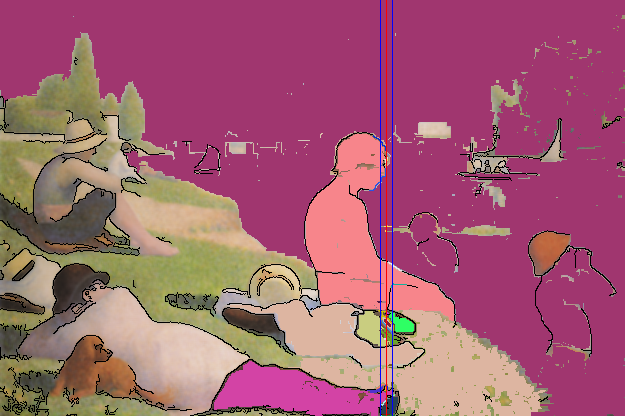
\includegraphics[scale=0.42,angle=0]{afsnit/afprovning/billeder/floodfillbilledet.png}
	\end{center}
	\caption[]{Billedet hvor vores algoritme har fundet x antal ragioner}
	\label{ff}
\end{figure}

I dette billedet er vær ragion, indtegnet med vær sin farve, og snittet
som er beregnet ud fra er det højensontale gyldne snit som ligger mest
til højre. Som man kan se finder algoritmen en masse ragioner, hvor
nogle af dem er ret spændne at se på, som f.eks. drengen som er farvet
helt lyserød. Der bliver også fundet en masse ragioner som ikke er
særlige spændne, f.eks. helle bagrunden som er malet mørke lilla i
billedet. Som man kan af billedet, er der ikke serlige mange ragioner, i
selve snittet som bliver tværet ud og kommer til at falde i et med et af
de andre ragioner i billedet, det er et godt tegn, da samelsmældingen af
ragioner vil give en forkert fortolkning af billedet.

Det andet naturlige sted at se på, er nå vi tager alle de fundenet ragioner om sotere dem fra, som ikke passer overens med vores defination af at ligge i snittet., ragioner som er taget med fra billedet \ref{ff}. 

\begin{figure}[h]
	\begin{center}
		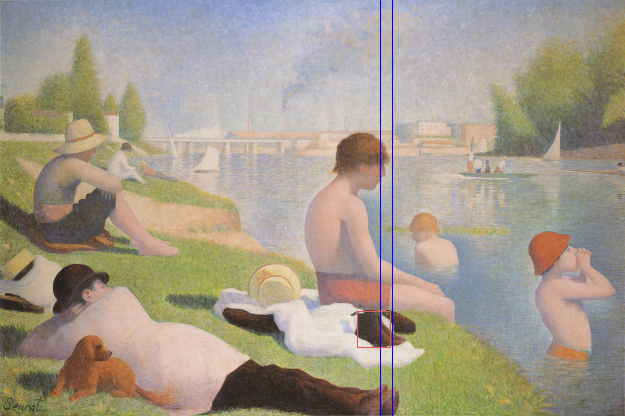
\includegraphics[scale=0.42,angle=0]{afsnit/afprovning/billeder/boindingboxbilledet.png}
	\end{center}
	\caption[]{Billedet de ragioner som vi har tilbage, er i en box}
	\label{blob}
\end{figure}

Som man kan se er der kun 1 ragion tilbage, som omkraser en sko i
billedet. Men tilgendgel er alle de store ragioner som bagrunden og
græset ikke blevet taget med. Det kan både siges at være godt og skidt.
det gode er at vi nu har en god ide om, hvad der bliver fundet. hvis vi
samme liner vores beskrivelse af vores fremgangsmåde, og hvordan
boilledet ser ud. Stemmer det over ens, så vores algoritme virker. Det
dårlige er, at vi fjerner ret meget. F.eks. kunne drengen være en
ragione som man gerne vil have med.

For at give lidt paspiktic, vil jeg også vise et andet billedet, hvor vores metode opføre sig en kænde anderledes.
	
 
\subsection{hvad kan vi gøre bedre}


\subsection{hvad er næste skrit}

% er der noget om at hvis man tegner et billedet, og der er noget i baggrunden, at de ting som er i bagrunden kommer til at få et skær af selve bagrunden
%problemstiullingen med thresholds
